\documentclass[11pt]{ctexart}
\usepackage[utf8]{inputenc}
\usepackage[left=1in,right=1in,top=1.2in,bottom=1.2in]{geometry}
\usepackage{fancyhdr}
\usepackage{amsmath}
\usepackage{amssymb}
\usepackage{multicol}
\usepackage{ctex}
\usepackage{hyperref}
\usepackage{listings}
\usepackage{xcolor}
\usepackage{graphicx,hyperref,url}
\usepackage{minted}
\usepackage{caption}
\usepackage{subfigure}
\usepackage{listings}
\usepackage{color}

\definecolor{dkgreen}{rgb}{0,0.6,0}
\definecolor{gray}{rgb}{0.5,0.5,0.5}
\definecolor{mauve}{rgb}{0.58,0,0.82}

\lstset{frame=tb,
  language=Python,
  aboveskip=3mm,
  belowskip=3mm,
  showstringspaces=false,
  columns=flexible,
  basicstyle={\small\ttfamily},
  numbers=none,
  numberstyle=\tiny\color{gray},
  keywordstyle=\color{blue},
  commentstyle=\color{dkgreen},
  stringstyle=\color{mauve},
  breaklines=true,
  breakatwhitespace=true,
  tabsize=3
}

% \usepackage{titlesec}
% \titlespacing\section{0pt}{15pt}{0pt}
% \titlespacing\subsection{0pt}{5pt}{0pt}
% \titlespacing\subsubsection{0pt}{5pt}{0pt}

\usepackage{enumitem}
\setlist{nolistsep}

\pagestyle{fancy}
\fancyhead[L]{East China Normal University}
\fancyhead[R]{\thepage}
\fancyfoot[C]{}

\fancypagestyle{plain}
{
\fancyhead[L]{East China Normal University}
\fancyhead[R]{\thepage}
\fancyfoot[C]{}
}

\ctexset{section/format=\Large\bfseries}



\setcounter{page}{1}

\title{华东师范大学软件工程实验报告}
\author{谢嘉东\ 10185101247\\陈俊潼\ 10185101210}
\date{March 2020}

\begin{document}

\maketitle

\thispagestyle{empty}

\begin{itemize}
    \item 课程名称:数字图像处理
    \item 年级:2018 级本科
    \item 实验编号:实验 002
    \item 上机实践日期:2020.3
\end{itemize}

\tableofcontents

\thispagestyle{empty}

\newpage

\section{分工情况}

组内两人共同查阅资料,完善代码,完成了实验部分和两道附加题。

实验报告由两人共同撰写。

\section{实验内容}

图像增强是指采用一系列技术改善图像的视觉效果,或将图像转换成一种更适合于人或机器进行分析处理的形式。图像增强并不以图像保真为准则,而是有选择地突出某些对人或机器分析有意义的信息,抑制无用信息,提高图像的使用价值。

图像分割是按照某些特性(如灰度级,频谱,纹理等)将图像划分成一些区域,在这些区域内其特性是相同的或者说是均匀的,两个相邻区域彼此特性则是不同的,其间存在着边缘或边界。图像分割从本质上来说是将图像中的像素按照特性的不同进行分类的过程。

本次实验本小组实现了图像增强的直方图均衡化和图像分割的边缘检测。分别使用 Laplachain 算子、Sobel 算子、Canny 算子导出结果。此外。同时对一幅肺部 CT 扫描图像分别通过巴特沃斯高通滤波器、高频强调和直方图均衡,得到了易于观察和诊断的图像。

\section{实验目的}

\begin{itemize}
    \item [1] 了解 Python OpenCV 库对图像的基本操作
    \item [2] 了解直方图的概念和含义
    \item [3] 掌握对图像进行直方图均衡和绘制直方图的具体操作
    \item [4] 理解不同的差分算子对图像分割的处理过程和具体实现
    \item [5] 探索在频率域上对图像进行通带滤波的原理和实现方法
\end{itemize}

\section{实验原理}

利用 numpy 、matplotlib.pyplot 、cv2 以及 Pillow 中的 PIL 包来辅助完成实验。其中主要用到了:

\begin{itemize}
    \item numpy.array(object, dtype=None, copy=True, order='K', subok=False, ndmin=0)
    \begin{itemize}
        \item object : array\_like
        \item dtype : data-type, optional
        \item copy : bool, optional
        \item order : {‘K’, ‘A’, ‘C’, ‘F’}, optional
        \item subok : bool, optional
        \item ndmin : int, optional
    \end{itemize}
    \item matplotlib.pyplot.hist(x, bins=None, range=None, density=False, weights=None, cumulative=False, bottom=None, histtype='bar', align='mid', orientation='vertical', rwidth=None, log=False, color=None, label=None, stacked=False, *, data=None, **kwargs)
    \item cv2.equalizeHist(src[, dst])
    \begin{itemize}
        \item src – Source 8-bit single channel image.
        \item dst – Destination image of the same size and type as src .
    \end{itemize}
    \item cv2.cvtColor(src, code[, dst[, dstCn]]) 
    \begin{itemize}
        \item src – input image.
        \item dst – output image of the same size and depth as src.
        \item code – color space conversion code.
        \item dstCn – number of channels in the destination image.
    \end{itemize}
    \item Laplacian( src\_gray, dst, ddepth, kernel\_size, scale, delta, BORDER\_DEFAULT );
    \begin{itemize}
        \item src\_gray: The input image.
        \item dst: Destination (output) image.
        \item ddepth: Depth of the destination image.
        \item kernel\_size: The kernel size of the Sobel operator to be applied internally.
        \item scale, delta and BORDER\_DEFAULT: We leave them as default values.
    \end{itemize}
    \item cv2.bitwise\_or(src1, src2[, dst[, mask]])
    \begin{itemize}
        \item src1 – first input array or a scalar.
        \item src2 – second input array or a scalar.
        \item dst – output array that has the same size and type as the input arrays.
        \item mask – optional operation mask, 8-bit single channel array.
    \end{itemize}
    \item cv2.Canny(image, threshold1, threshold2[, edges[, apertureSize[, L2gradient]]])
    \begin{itemize}
        \item image – single-channel 8-bit input image.
        \item threshold1 – first threshold for the hysteresis procedure.
        \item threshold2 – second threshold for the hysteresis procedure.
        \item edges – output edge map; it has the same size and type as image .
        \item apertureSize – aperture size for the Sobel() operator.
    \end{itemize}
    \item numpy.fft.ifft(a, n=None, axis=-1, norm=None)
    \begin{itemize}
        \item a : array\_like
        \item n : int, optional
        \item axis : int, optional
        \item norm : {None, “ortho”}, optional
    \end{itemize}
\end{itemize}

\section{实验方法}

\subsection{绘制图像直方图}

之后的众多步骤都需要利用直方图来辅助分析,所以我们实验的第一步是实现直方图的绘制。

为了可以统一化地绘制直方图,我们绘制的步骤是:

\begin{itemize}
    \item [1] 将输入的图片转换成灰度图
    \item [2] 统计图片中每一个灰度级出现的次数
    \item [3] 利用 matplotlib.pyplot 中的 hist 函数绘制图表
\end{itemize}

  \begin{figure}[htbp]
        \centering
        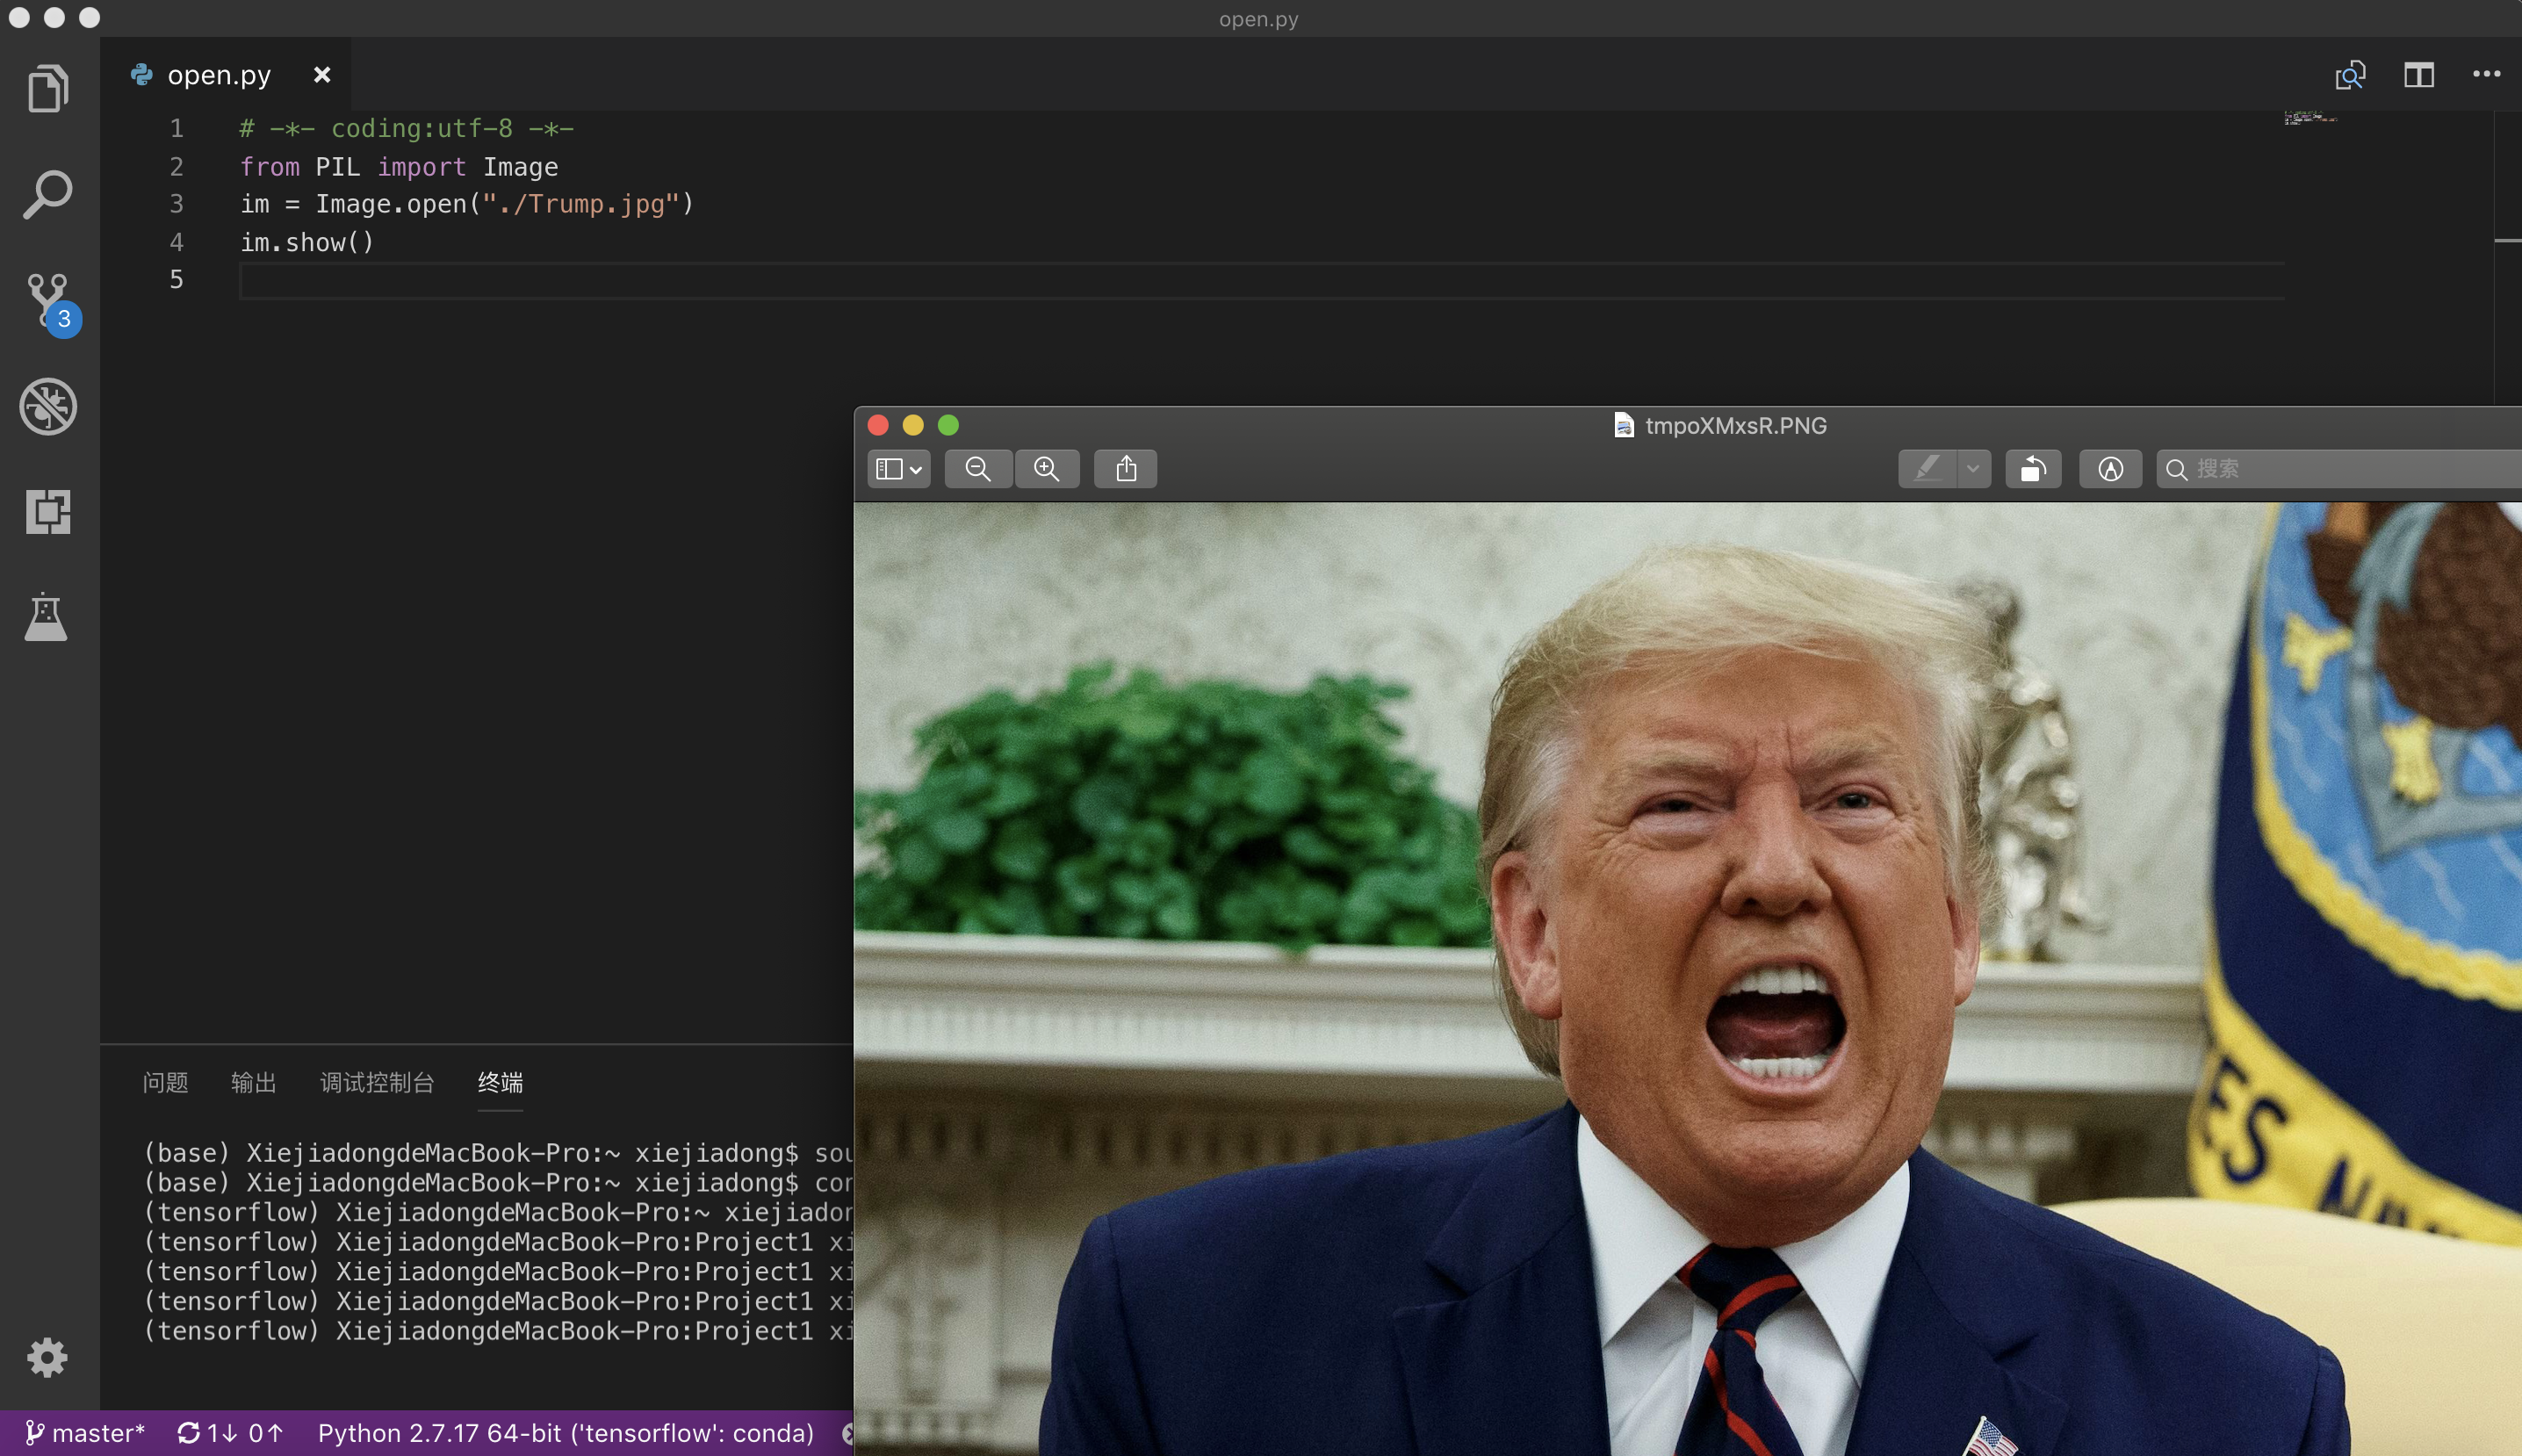
\includegraphics[width=0.6\textwidth]{./img/pic1.png}
        \caption{绘制直方图效果图}\label{fig:digit}
  \end{figure}

\subsection{直方图均衡化}

直方图均衡化中,我们针对两种不同的图片实现直方图均衡化。

\paragraph{灰度图直方图均衡化}

灰度图的直方图比较方便,我们直接利用 cv2 的 equalizeHist 函数,对输入的灰度图进行直方图均衡化后输出即可。

\paragraph{彩色图片直方图均衡化}

彩色图片直方图均衡化,对于简单的 RGB 彩色图像,如果直接分离三种颜色分别直方图均衡化是不会产生效果的。因为直方图的均衡化涉及强度图像的值,而不是颜色分量。因此,对于简单的 RGB 彩色图像,为了不干扰图像的颜色平衡,我们先将图像的颜色空间从 RGB 转换为 YCbCr 颜色空间,该空间将灰度值与颜色分量分离。之后再采用 cv2 的 equalizeHist 函数,将图片进行直方图均衡化,之后将图片转变回 RGB 彩色图像,输出图片。

\subsection{差分算子边缘检测}

我们使用了 Laplacian 和 Sobel 两种不同的差分算子进行了边缘检测。

\paragraph{Laplacian}

这部分比较方便处理,只需要将图片转变成灰度图片,然后直接利用 cv2 的 Laplacian 进行计算。

\paragraph{Sobel}

与 Laplacian 不同的是,Sobel 还涉及到差分的方向问题。我们分别对图片计算了 $x$ 方向的梯度和 $y$ 方向的梯度,之后对这两部分的计算进行了合并得到了最后的边缘检测结果。

\subsection{Canny 算子边缘检测}

首先,由于 Canny 只能处理灰度图,所以将读取的图像转成灰度图。Canny 算子涉及到两个阀值,通过查阅相关的资料了解到,较大的阈值用于检测图像中明显的边缘,但一般情况下检测的效果不会那么完美,边缘检测出来会是断断续续的。所以这时候我们需要用较小的第一个阈值用于将这些间断的边缘连接起来。

我们尝试了一些不同的阀值来输出图片,比较他们的结果。

\subsection{巴特沃斯高通滤波与高频强调(频率域处理)}

为了实现巴特沃斯高通滤波与高频强调,需要在频率域处理图像。巴特沃斯滤波器的阶数会影响到频率的相应曲线,通常采用 2 阶即可取得较好结果并避免振铃效应。

  \begin{figure}[htbp]
        \centering
        \includegraphics[width=0.6\textwidth]{butterworth.png}
        \caption{巴特沃斯低通滤波器的频率响应曲线}\label{fig:digit}
  \end{figure}
  
设图像的中心为 $(m, n)$,$D(u, v)$ 表示图像到中心点的距离,$H(u, v)$ 为输出的频率,$M$ 和 $N$ 表示图像的长度与宽度, $D_{0}$ 表示截频宽度,$n$ 表示阶数,则巴特沃斯低通滤波器的传递函数为:

$$
H(u, v) = \frac{1}{1 + (D_{0} / D(u, v))^{2n}}
$$

相应的有巴特沃斯高通滤波器传递函数为:
$$
H(u, v) = \frac{1}{1 + (D(u, v) / D_{0})^{2n}}
$$

其中 $D(u, v)$ 表示振幅,即像素偏离图像中心的距离:

$$
D(u, v) = \sqrt{(u - m)^2 - (v - n)^2}
$$

为了在频率域处理图像,先采用 numpy 库的 fft 和 fftshift 方法对图像进行二维傅里叶变换并频移动至中心。接着对频率域中的每个像素使用巴特沃斯高通滤波器的公式进行处理即可。图像的低频部分集中在频率域的中心,高频部分集中在频率域的四周。利用巴特沃斯高通滤波器过滤掉中心的部分低频,再将图像逆傅里叶变换还原。

在还原之后,由于原图像灰度过低不易观察,我们将整体图像的灰度提高了 60。

 \begin{figure}[htbp]
        \centering
        \subfigure[频率域图像]{
            \begin{minipage}[t]{0.45\linewidth}
            \centering
             \includegraphics[width=0.6\textwidth]{9_A_fft.jpg}
            \end{minipage}
        }
        \subfigure[经巴特沃斯高通滤波]{
            \begin{minipage}[t]{0.45\linewidth}
            \centering
             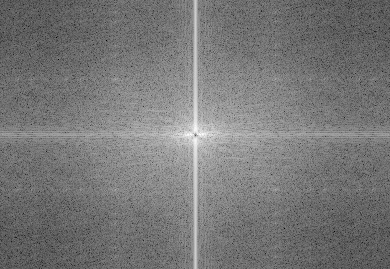
\includegraphics[width=0.6\textwidth]{9_A_Processing.jpg}
            \end{minipage}
        }
        \caption{频率域处理}\label{fig:digit}
  \end{figure}

为了实现高频强调,只需在频率域的图像进行巴特沃斯滤波处理时,每个像素都经过线性增益即可。高频强调滤波器的传递函数为:

$$
H_{hfe}(u, v) = a + bH_{hp}(u, v)
$$


这里采用的参数是 $H = 1.5 + 0.5H$,经过该处理得到 C 图像,最后再调用直方图均衡函数 cv2.euqalizeHist() 即可得到 D。

\section{实验结果及分析}

基本完成了实验预期所要达到的要求。

最终的实验结果如下:

\subsection*{直方图均衡化}

\subsubsection*{灰度图}

    \begin{figure}[htbp]
        \centering
        \subfigure[原图]{
            \begin{minipage}[t]{0.4\linewidth}
            \centering
            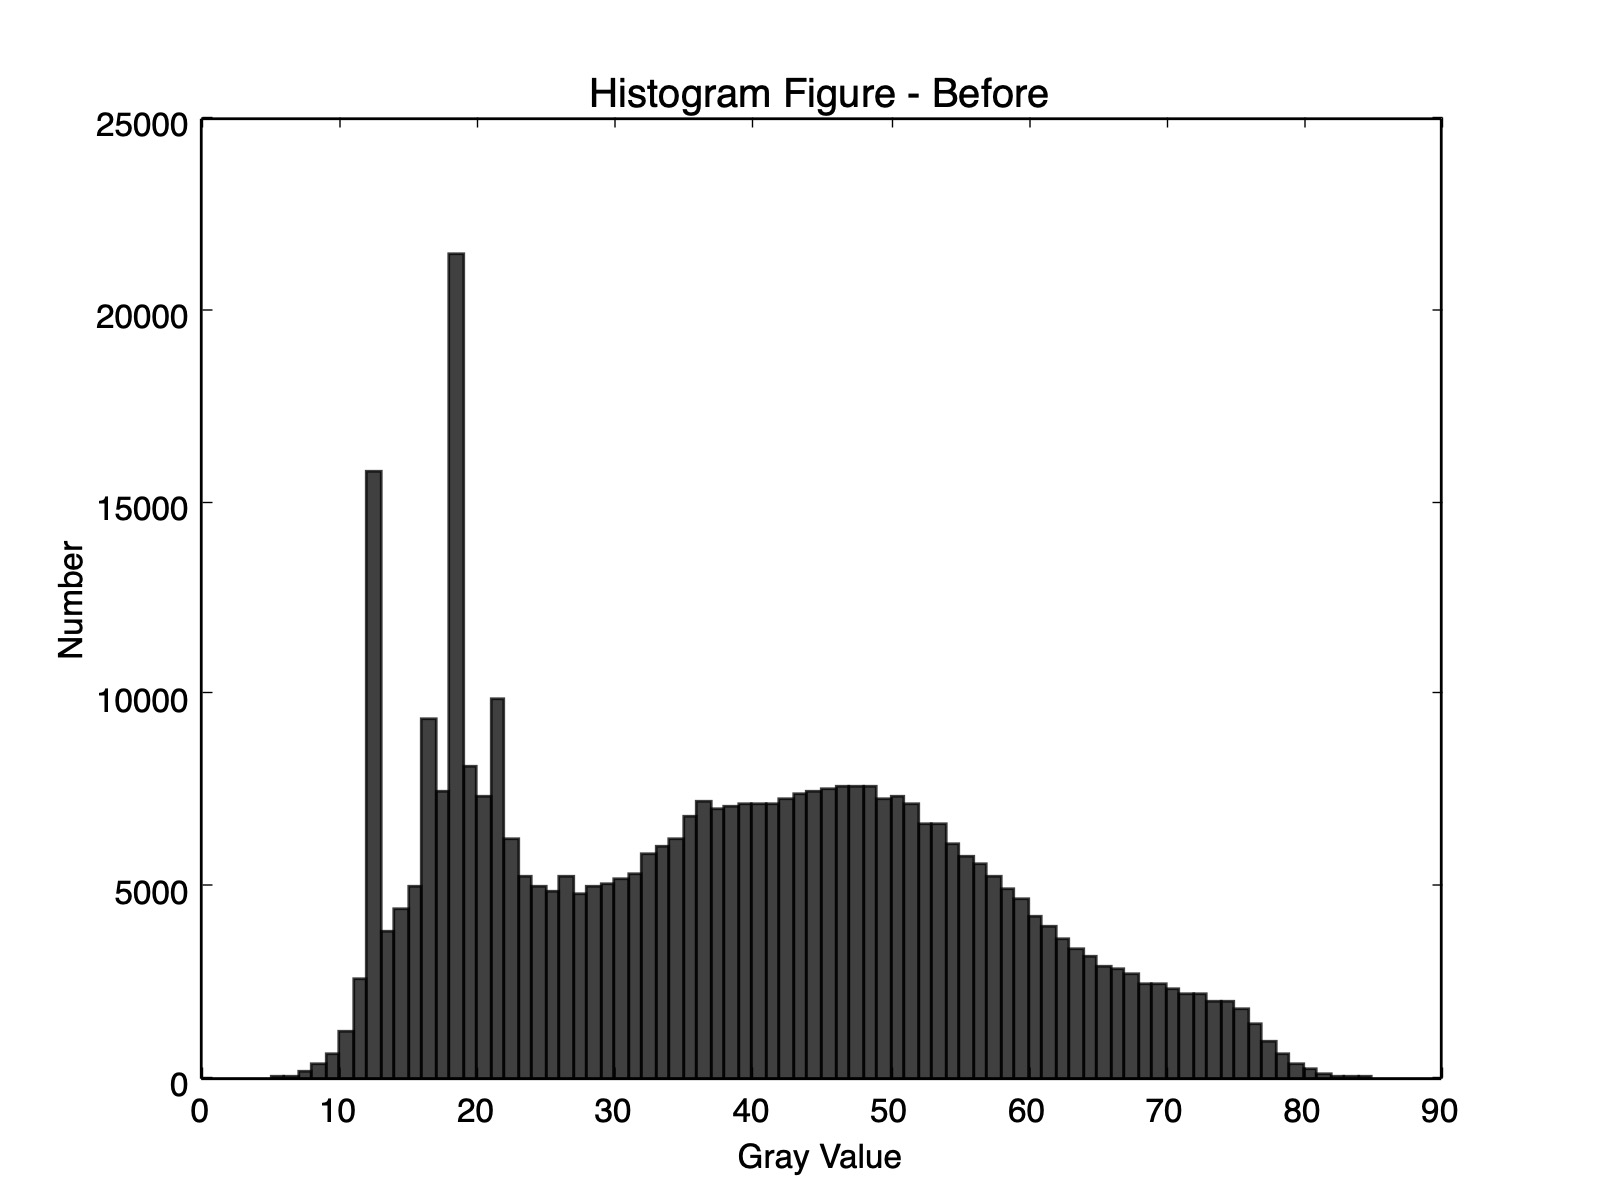
\includegraphics[width=0.6\textwidth]{./3_before.jpg}
        \end{minipage}
        }
        \subfigure[直方图均衡化结果]{
            \begin{minipage}[t]{0.4\linewidth}
            \centering
            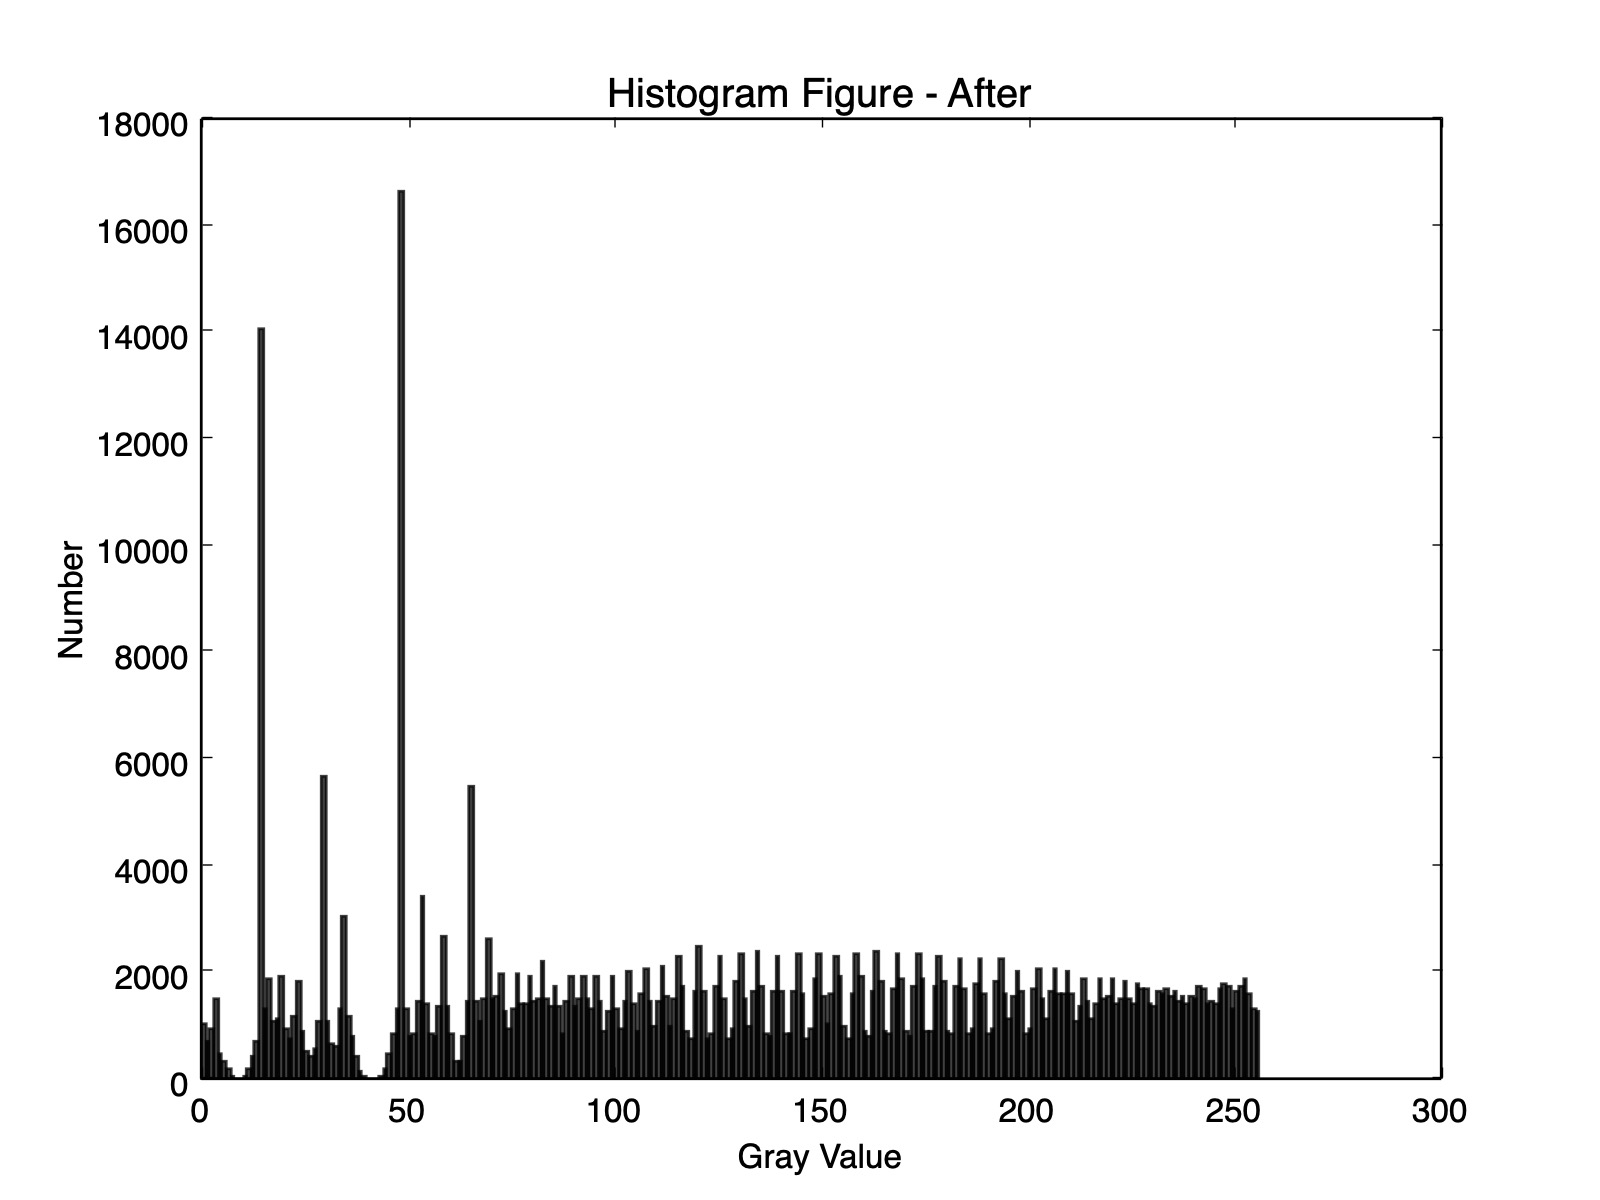
\includegraphics[width=0.6\textwidth]{./3_after.jpg}
            \end{minipage}
        }
        \centering
        \caption{处理前后直方图对比}\label{fig:digit}
  \end{figure}

    \begin{figure}[htbp]
        \centering
        \subfigure[原图]{
            \begin{minipage}[t]{0.4\linewidth}
            \centering
            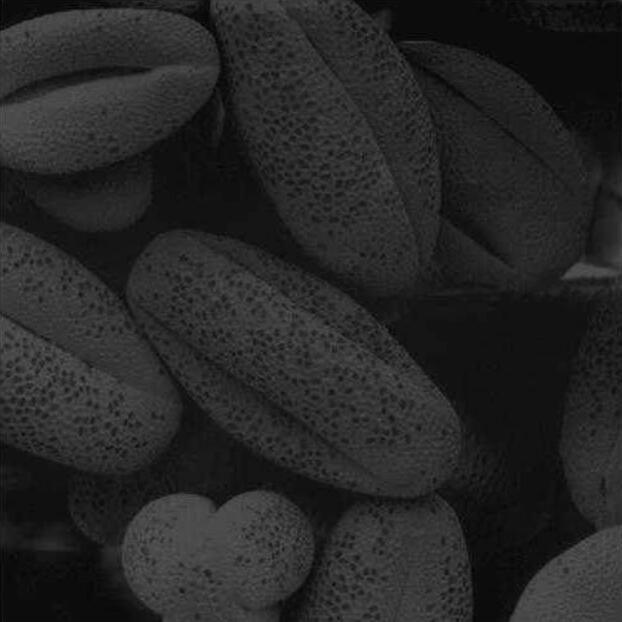
\includegraphics[width=0.6\textwidth]{./3_input.jpg}
        \end{minipage}
        }
        \subfigure[直方图均衡化结果]{
            \begin{minipage}[t]{0.4\linewidth}
            \centering
            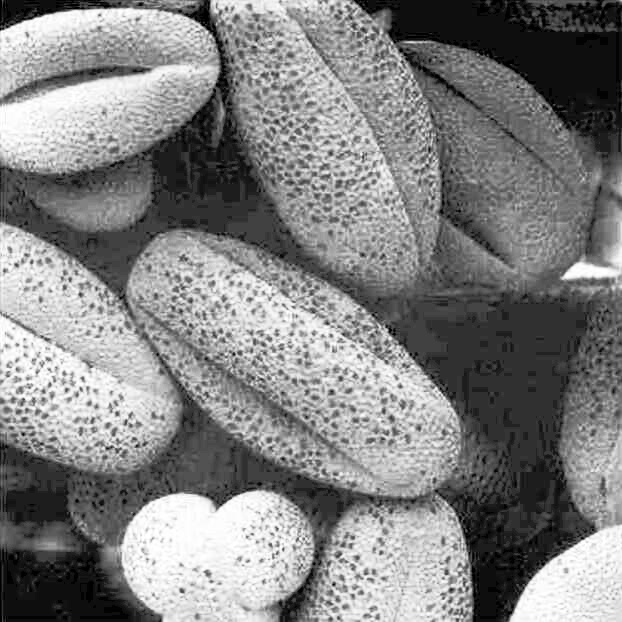
\includegraphics[width=0.6\textwidth]{./3_equalize_histogram.jpg}
            \end{minipage}
        }
        \centering
        \caption{直方图均衡化}\label{fig:digit}
  \end{figure}

  \newpage

\subsubsection*{彩色图}

    \begin{figure}[htbp]
        \centering
        \subfigure[原图]{
            \begin{minipage}[t]{0.4\linewidth}
            \centering
            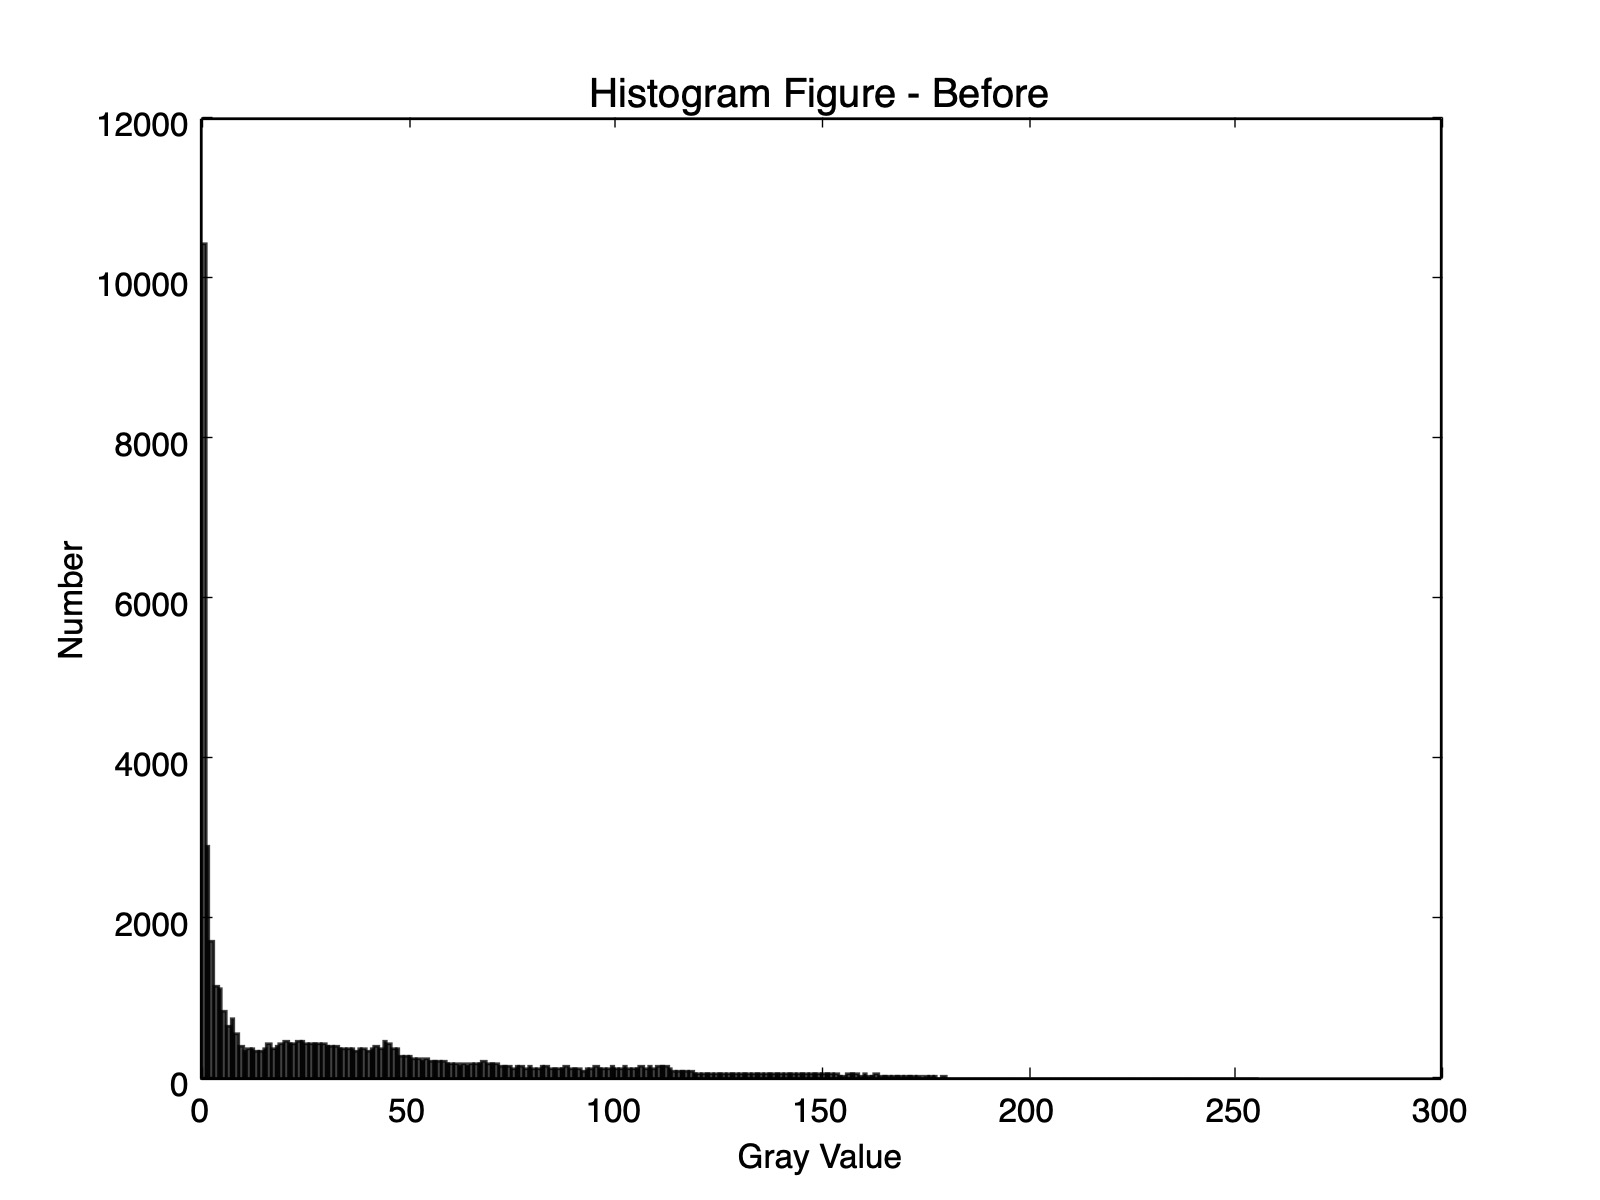
\includegraphics[width=0.6\textwidth]{./3_before_color.jpg}
        \end{minipage}
        }
        \subfigure[直方图均衡化结果]{
            \begin{minipage}[t]{0.4\linewidth}
            \centering
            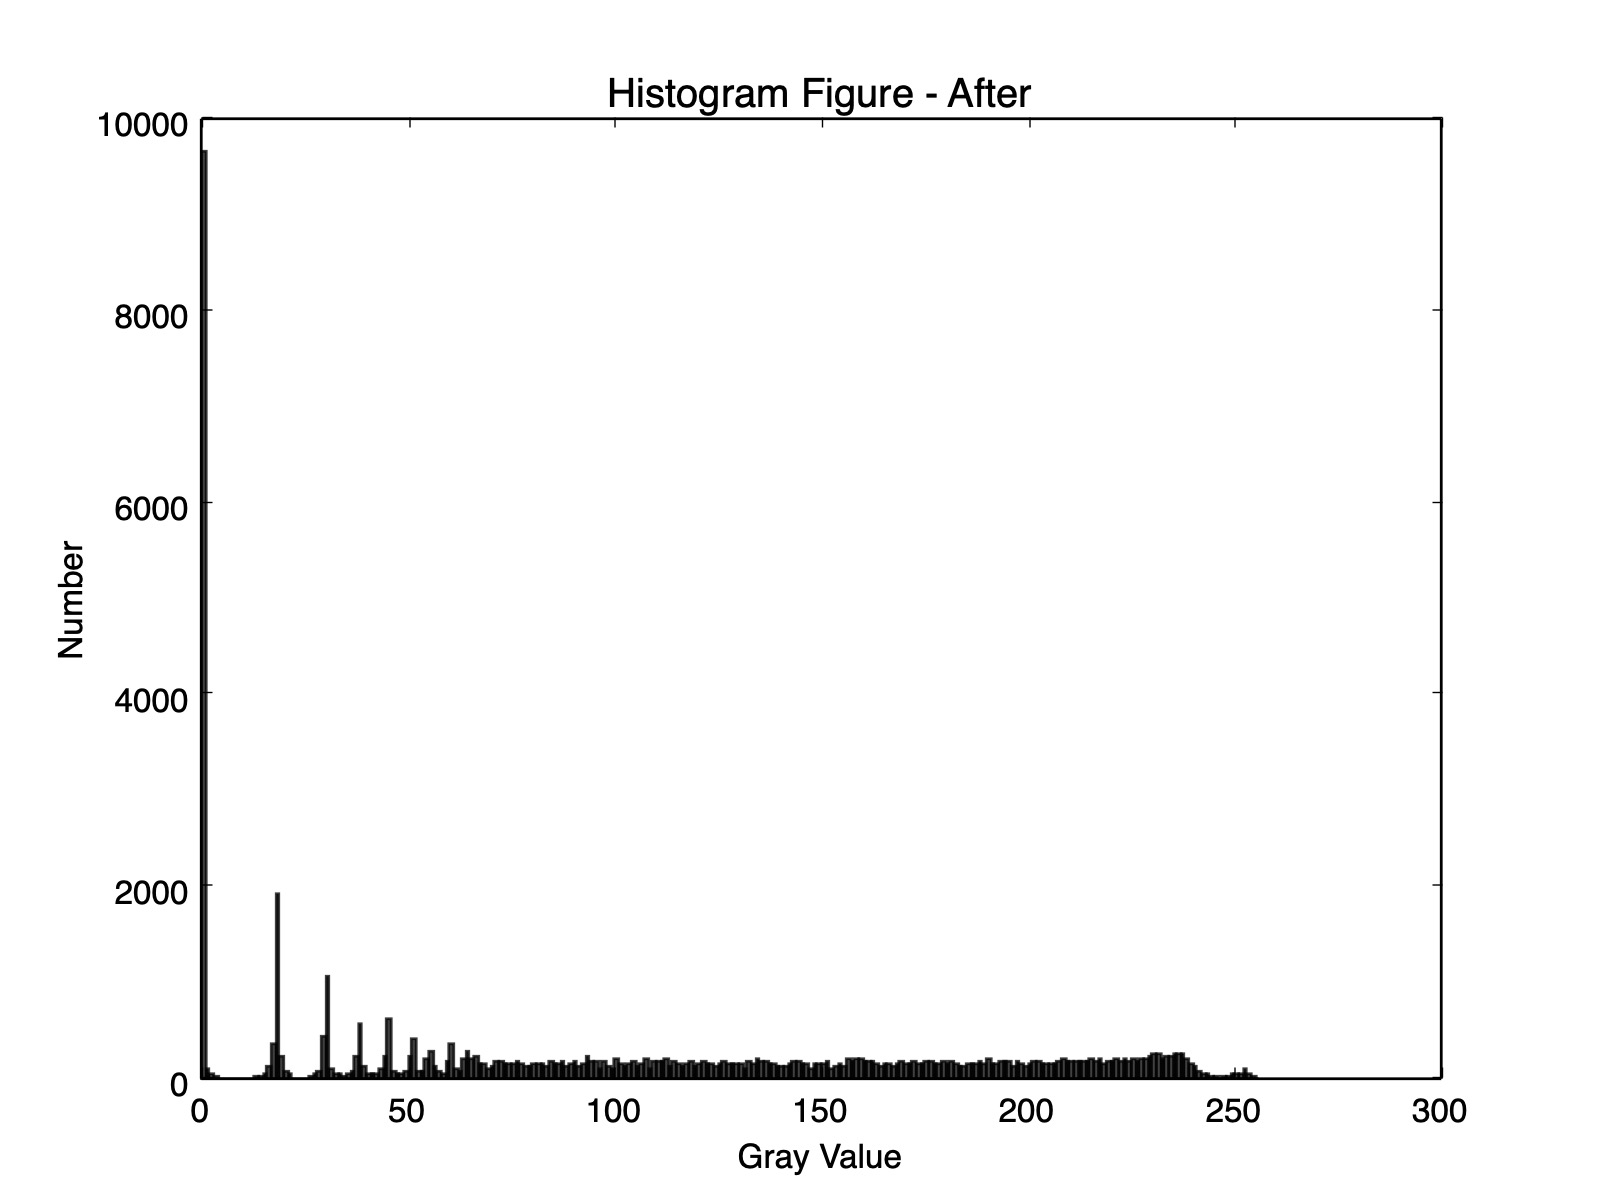
\includegraphics[width=0.6\textwidth]{./3_after_color.jpg}
            \end{minipage}
        }
        \centering
        \caption{处理前后直方图对比}\label{fig:digit}
  \end{figure}
  

    \begin{figure}[htbp]
        \centering
        \subfigure[原图]{
            \begin{minipage}[t]{0.4\linewidth}
            \centering
            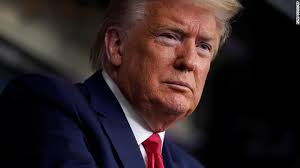
\includegraphics[width=0.6\textwidth]{./3_input_color.jpeg}
        \end{minipage}
        }
        \subfigure[直方图均衡化结果]{
            \begin{minipage}[t]{0.4\linewidth}
            \centering
            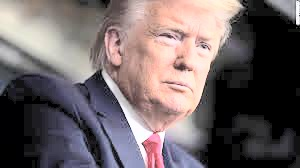
\includegraphics[width=0.6\textwidth]{./3_equalize_histogram_color.jpg}
            \end{minipage}
        }
        \centering
        \caption{直方图均衡化}\label{fig:digit}
  \end{figure}
  
\subsection* {差分算子边缘检测}

\subsubsection*{Laplacian}


    \begin{figure}[htbp]
        \centering
        \subfigure[原图]{
            \begin{minipage}[t]{0.4\linewidth}
            \centering
            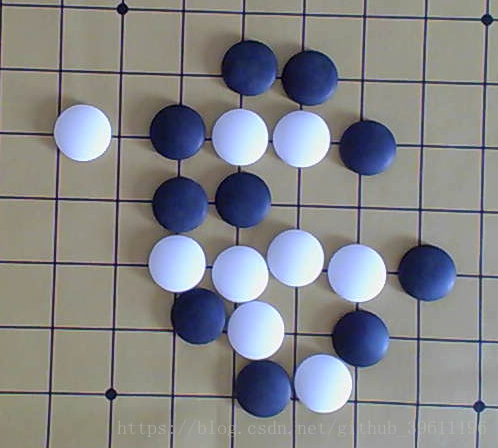
\includegraphics[width=0.6\textwidth]{./6_edge_detection_2.png}
        \end{minipage}
        }
        \subfigure[边缘检测]{
            \begin{minipage}[t]{0.4\linewidth}
            \centering
            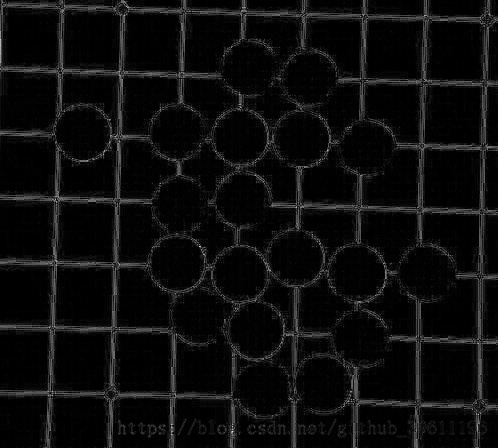
\includegraphics[width=0.6\textwidth]{./6_Laplacian_2.jpg}
            \end{minipage}
        }
        \centering
        \caption{Laplacian}\label{fig:digit}
  \end{figure}
  
 \newpage
 
      \begin{figure}[htbp]
        \centering
        \subfigure[原图]{
            \begin{minipage}[t]{0.4\linewidth}
            \centering
            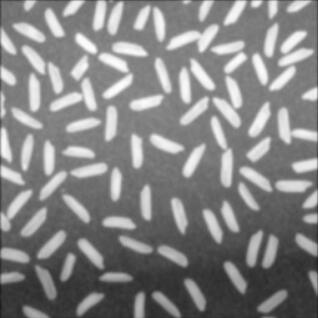
\includegraphics[width=0.5\textwidth]{./6_edge_detection_1.jpg}
        \end{minipage}
        }
        \subfigure[边缘检测]{
            \begin{minipage}[t]{0.4\linewidth}
            \centering
            
\includegraphics[width=0.5\textwidth]{./6_Laplacian_1.jpg}
            \end{minipage}
        }
        \centering
        \caption{Laplacian}\label{fig:digit}
  \end{figure}
  
\subsubsection*{Sobel}


      \begin{figure}[htbp]
        \centering
        \subfigure[原图]{
            \begin{minipage}[t]{0.4\linewidth}
            \centering
            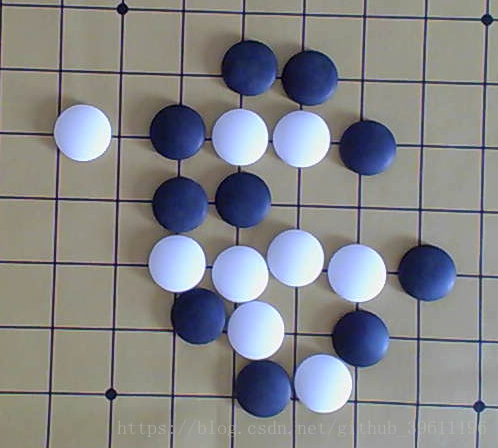
\includegraphics[width=0.6\textwidth]{./6_edge_detection_2.png}
        \end{minipage}
        }
        \subfigure[合成后的结果]{
            \begin{minipage}[t]{0.4\linewidth}
            \centering
            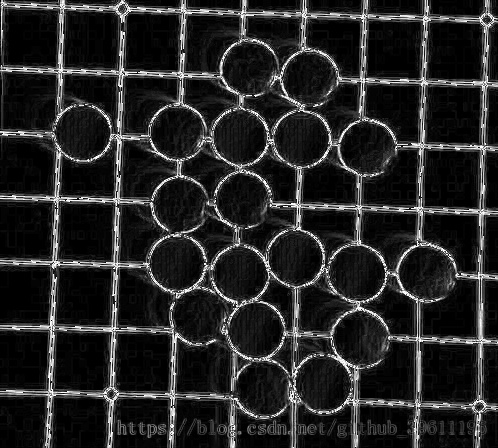
\includegraphics[width=0.6\textwidth]{./6_Sobel_2_combined.jpg}
            \end{minipage}
        }
        \subfigure[X 方向检测]{
            \begin{minipage}[t]{0.4\linewidth}
            \centering
            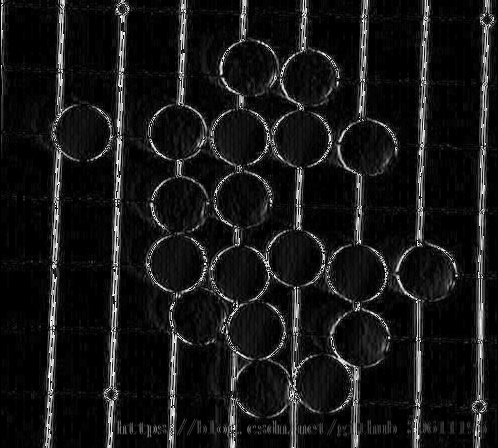
\includegraphics[width=0.6\textwidth]{./6_Sobel_2_X.jpg}
            \end{minipage}
        }
        \subfigure[Y 方向检测]{
            \begin{minipage}[t]{0.4\linewidth}
            \centering
            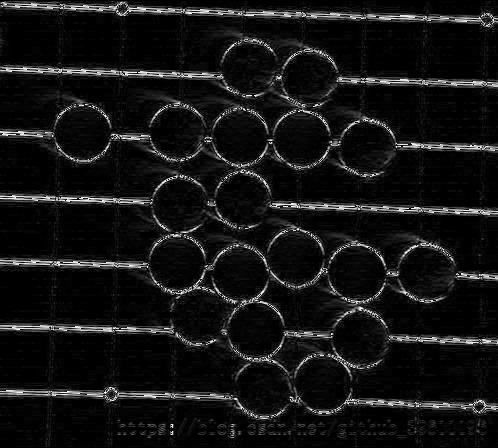
\includegraphics[width=0.6\textwidth]{./6_Sobel_2_Y.jpg}
            \end{minipage}
        }
        \centering
        \caption{Sobel}\label{fig:digit}
  \end{figure}

\newpage
 
      \begin{figure}[htbp]
        \centering
        \subfigure[原图]{
            \begin{minipage}[t]{0.4\linewidth}
            \centering
            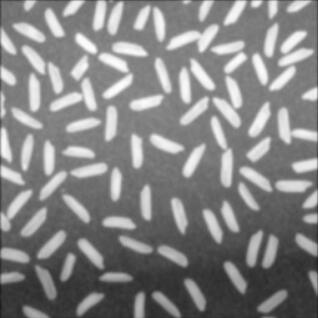
\includegraphics[width=0.5\textwidth]{./6_edge_detection_1.jpg}
        \end{minipage}
        }
        \subfigure[合成后的结果]{
            \begin{minipage}[t]{0.4\linewidth}
            \centering
            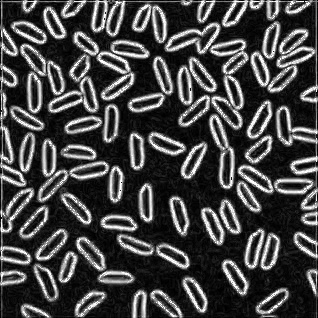
\includegraphics[width=0.5\textwidth]{./6_Sobel_1_combined.jpg}
            \end{minipage}
        }
        \subfigure[X 方向检测]{
            \begin{minipage}[t]{0.4\linewidth}
            \centering
            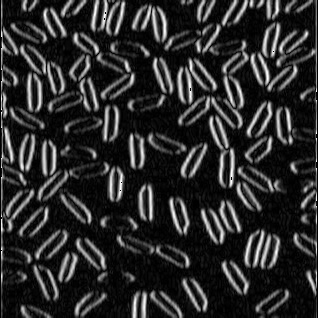
\includegraphics[width=0.5\textwidth]{./6_Sobel_1_X.jpg}
            \end{minipage}
        }
        \subfigure[Y 方向检测]{
            \begin{minipage}[t]{0.4\linewidth}
            \centering
            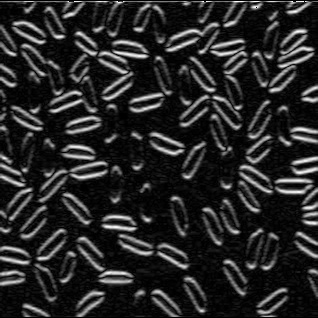
\includegraphics[width=0.5\textwidth]{./6_Sobel_1_Y.jpg}
            \end{minipage}
        }
        \centering
        \caption{Sobel}\label{fig:digit}
  \end{figure}
  
\subsection*{Canny}

      \begin{figure}[htbp]
        \centering
        \subfigure[threshold1=10,threshold2=250]{
            \begin{minipage}[t]{0.4\linewidth}
            \centering
            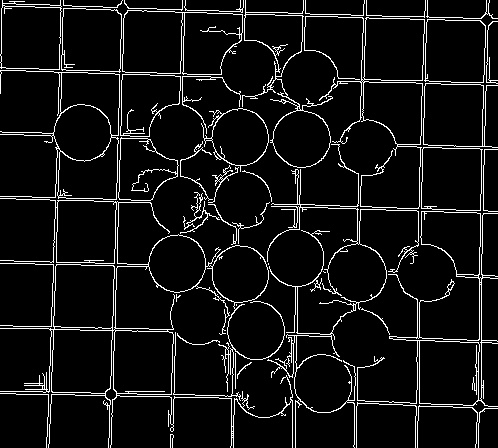
\includegraphics[width=0.5\textwidth]{./8_Canny_2_10_250_2.jpg}
        \end{minipage}
        }
        \subfigure[threshold1=30,threshold2=150]{
            \begin{minipage}[t]{0.4\linewidth}
            \centering
            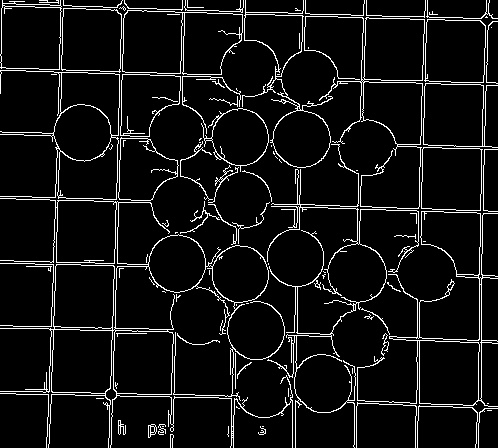
\includegraphics[width=0.5\textwidth]{./8_Canny_2_30_150_2.jpg}
            \end{minipage}
        }
        \centering
        \caption{Canny}\label{fig:digit}
  \end{figure}

      \begin{figure}[htbp]
        \centering
        \subfigure[threshold1=30,threshold2=250]{
            \begin{minipage}[t]{0.4\linewidth}
            \centering
            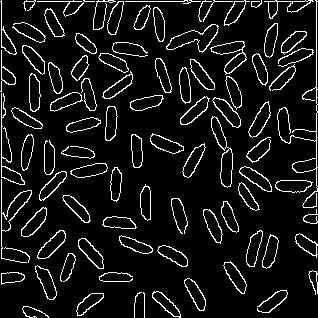
\includegraphics[width=0.5\textwidth]{./8_Canny_1_30_250_2.jpg}
            \end{minipage}
        }
        \subfigure[threshold1=30,threshold2=200]{
            \begin{minipage}[t]{0.4\linewidth}
            \centering
            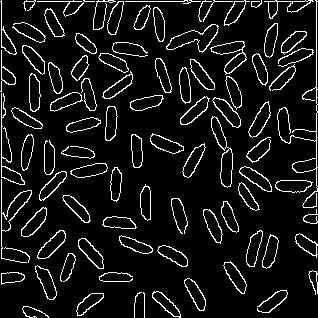
\includegraphics[width=0.5\textwidth]{./8_Canny_1_30_200_2.jpg}
            \end{minipage}
        }
        \centering
        \caption{Canny}\label{fig:digit}
  \end{figure}
  
  \newpage
  
\subsection*{巴特沃斯滤波器与高频强调(医学图像处理)}

     \begin{figure}[htbp]
        \centering
        \subfigure[原图]{
            \begin{minipage}[t]{0.4\linewidth}
            \centering
            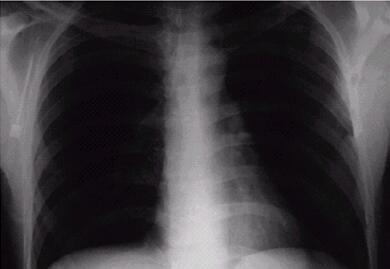
\includegraphics[width=0.6\textwidth]{./9_input.jpg}
        \end{minipage}
        }
        \subfigure[Butterworth Highpass Filter]{
            \begin{minipage}[t]{0.4\linewidth}
            \centering
            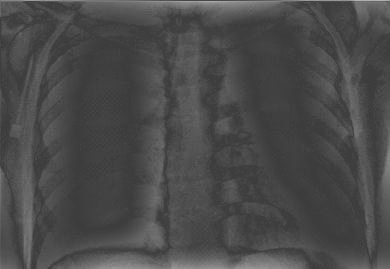
\includegraphics[width=0.6\textwidth]{./9_B.jpg}
            \end{minipage}
        }
        \subfigure[High Freguency Emphasis]{
            \begin{minipage}[t]{0.4\linewidth}
            \centering
            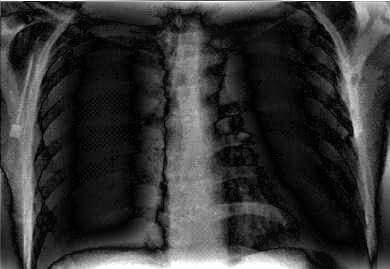
\includegraphics[width=0.6\textwidth]{./9_C.jpg}
            \end{minipage}
        }
        \subfigure[Histogram Equalization]{
            \begin{minipage}[t]{0.4\linewidth}
            \centering
            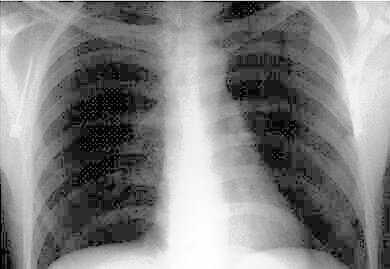
\includegraphics[width=0.6\textwidth]{./9_D.jpg}
            \end{minipage}
        }
        \centering
        \caption{医学图像处理}\label{fig:digit}
  \end{figure}
  
  
\section{主要核心代码}

\paragraph{绘制图像直方图}

\lstset{language=python}
\begin{lstlisting}
# encoding:utf-8
import matplotlib.pyplot as plt
import numpy as np
from PIL import Image

#drawHistogram 函数用来画直方图
def drawHistogram(input, output, title = ''):
	#导入图像
	img = Image.open(input)
	#将图像转换成灰度图像
	img = img.convert('L')
	#统计每种灰度出现的次数
	arr = np.array(img).flatten()
	print(len(arr))
	#绘制直方图,设置 x/y 轴相关参数和图标标题
	plt.hist(arr, bins=256, facecolor='black', alpha=0.75, range=[0, 256])
	plt.xlabel('Gray Value')
	plt.ylabel('Number')
	plt.title(title)
	plt.savefig(output)
	plt.show()

#分别绘制处理前后的直方图
drawHistogram('input/3_input.jpg', 'output/3_before.jpg', "Histogram Figure - Before")
drawHistogram('output/3_equalize_histogram.jpg', 'output/3_after.jpg', "Histogram Figure - After")

drawHistogram('input/3_input_color.jpeg', 'output/3_before_color.jpg', "Histogram Figure - Before")
drawHistogram('output/3_equalize_histogram_color.jpg', 'output/3_after_color.jpg', "Histogram Figure - After")
\end{lstlisting}

\paragraph{直方图均衡化}

\lstset{language=python}
\begin{lstlisting}
# coding=utf-8
import cv2

#灰度图直方图均衡化
def equalizeHistogram(input, output):
	img = cv2.imread(input, 0)
	#对输入灰度图直方图均衡化
	equ = cv2.equalizeHist(img)
	#保存均衡化后的结果
	cv2.imwrite(output, equ, [int(cv2.IMWRITE_JPEG_QUALITY), 95])

#彩色图直方图均衡化
def equalizeHistogramRGB(input, output):
	img = cv2.imread(input)
	#读取图像并转换为 YCbCr 色彩空间
	ycrgb = cv2.cvtColor(img, cv2.COLOR_BGR2YCR_CB)
	channels = cv2.split(ycrgb)
	#将图片直方图均衡化
	cv2.equalizeHist(channels[0], channels[0])
	cv2.merge(channels, ycrgb)
	#将图片转变回 RGB 色彩空间
	cv2.cvtColor(ycrgb, cv2.COLOR_YCR_CB2BGR, img)
	#保存均衡化后的结果
	cv2.imwrite(output, img, [int(cv2.IMWRITE_JPEG_QUALITY), 95])

equalizeHistogram('input/3_input.jpg', 'output/3_equalize_hisyogram.jpg')
equalizeHistogramRGB('input/3_input_color.jpeg', 'output/3_equalize_histogram_color.jpg')
\end{lstlisting}

\paragraph{差分算子边缘检测}

\lstset{language=python}
\begin{lstlisting}
# encoding:utf-8
import cv2
import numpy as np

def Laplacian(input, output):
	Image = cv2.imread(input)
	# 将图像转化为灰度图像
	Image = cv2.cvtColor(Image, cv2.COLOR_BGR2GRAY)
	# 拉普拉斯边缘检测
	lap = cv2.Laplacian(Image, cv2.CV_64F)
	# 对 lap 取绝对值
	lap = np.uint8(np.absolute(lap))
	cv2.imshow("Laplacian", lap)
	cv2.imwrite(output, lap, [int(cv2.IMWRITE_JPEG_QUALITY), 95])

def Sobel(input, output):
	Image = cv2.imread(input)
	# 将图像转化为灰度图像
	Image = cv2.cvtColor(Image, cv2.COLOR_BGR2GRAY)
	# Sobel边缘检测
	# x方向的梯度
	sobelX = cv2.Sobel(Image, cv2.CV_64F, 1, 0)
	# y方向的梯度
	sobelY = cv2.Sobel(Image, cv2.CV_64F, 0, 1)
	# x方向梯度的绝对值
	sobelX = np.uint8(np.absolute(sobelX))
	# y方向梯度的绝对值
	sobelY = np.uint8(np.absolute(sobelY))
	# 联合两部分边缘检测
	sobelCombined = cv2.bitwise_or(sobelX, sobelY)
	cv2.imwrite(output.replace('.jpg', '') + '_X.jpg', sobelX, [int(cv2.IMWRITE_JPEG_QUALITY), 95])
	cv2.imwrite(output.replace('.jpg', '') + '_Y.jpg', sobelY, [int(cv2.IMWRITE_JPEG_QUALITY), 95])
	cv2.imwrite(output.replace('.jpg', '') + '_combined.jpg', sobelCombined, [int(cv2.IMWRITE_JPEG_QUALITY), 95])


Laplacian('input/6_edge_detection_1.jpg', 'output/6_Laplacian_1.jpg')
Laplacian('input/6_edge_detection_2.png', 'output/6_Laplacian_2.jpg')
Sobel('input/6_edge_detection_1.jpg', 'output/6_Sobel_1.jpg')
Sobel('input/6_edge_detection_2.png', 'output/6_Sobel_2.jpg')
\end{lstlisting}

\paragraph{Canny}

\lstset{language=python}
\begin{lstlisting}
# encoding:utf-8
import cv2

thresholds = [
	(30, 150),
	(10, 250),
	(30, 200),
	(30, 250)
]

def Canny(input, output):
	Image = cv2.imread(input)
	# 将图像转化为灰度图像
	Image = cv2.cvtColor(Image, cv2.COLOR_BGR2GRAY)
	# Canny边缘检测s
	for para in thresholds:
		canny = cv2.Canny(Image, para[0], para[1])
		cv2.imwrite(output.replace('.jpg', '') + '_' + str(para[0]) + '_'+ str(para[1]) + '_2.jpg',
		            canny, [int(cv2.IMWRITE_JPEG_QUALITY), 95])

Canny('input/6_edge_detection_1.jpg', 'output/8_Canny_1.jpg')
Canny('input/6_edge_detection_2.png', 'output/8_Canny_2.jpg')
\end{lstlisting}

\paragraph{巴特沃斯滤波器与高频强调(频率域处理)}

\lstset{language=python}
\begin{lstlisting}
import cv2
import numpy as np
def ButterworthHighPass(img):
	# 傅立叶变换
	f = np.fft.fft2(img)
	# 频移至中心
	img = np.fft.fftshift(f)
	# 指定截止频率为宽度的 1.5 %
	D0 = img.shape[0] * 0.015
	# 指定巴特沃斯滤波器的阶数
	frac = 2
	# 指定中点 (M, N)
	M = img.shape[0] / 2
	N = img.shape[1] / 2
	for v in range(img.shape[1]):
		for u in range(img.shape[0]):
			D = np.sqrt(np.square(u - M) + np.square(v - N))
			H = 1 / (1 + np.power((D0 / D), 2 * frac))
			img[u][v] = img[u][v] * H
	cv2.imwrite('output/9_A_Processing.jpg', 20 * np.log(np.abs(img)), [int(cv2.IMWRITE_JPEG_QUALITY), 95])
	# 逆傅立叶变换
	inversed = np.fft.ifft2(np.fft.ifftshift(img))
	# 为了让背景更明显
	inversed = np.abs(inversed) + 60
	return inversed

def HighFrequencyEmphasis(img):
	# 和 Butterworth 相比而言多了一步
	# 傅立叶变换
	f = np.fft.fft2(img)
	# 频移至中心
	img = np.fft.fftshift(f)
	# 指定截止频率为宽度的 1.5 %
	D0 = img.shape[0] * 0.05
	# 指定巴特沃斯滤波器的阶数
	frac = 2
	# 指定中点 (M, N)
	M = img.shape[0] / 2
	N = img.shape[1] / 2
	for v in range(img.shape[1]):
		for u in range(img.shape[0]):
			D = np.sqrt(np.square(u - M) + np.square(v - N))
			H = 1 / (1 + np.power((D0 / D), 2 * frac))
			# High Frequency Emphasis
			H = 0.5 + 1.5 * H
			img[u][v] = img[u][v] * H
	cv2.imwrite('output/9_A_Processing.jpg', 20 * np.log(np.abs(img)), [int(cv2.IMWRITE_JPEG_QUALITY), 95])
	# 逆傅立叶变换
	inversed = np.fft.ifft2(np.fft.ifftshift(img))
	inversed = np.abs(inversed)
	return inversed


def equalizeHistogram(img):
	img = np.uint8(img)
	equ = cv2.equalizeHist(img)
	return equ

img = cv2.imread('input/9_input.jpg')
img = cv2.cvtColor(img, cv2.COLOR_BGR2GRAY)
B = ButterworthHighPass(img)
cv2.imwrite('output/9_B.jpg', B, [int(cv2.IMWRITE_JPEG_QUALITY), 95])
C = HighFrequencyEmphasis(img)
cv2.imwrite('output/9_C.jpg', C, [int(cv2.IMWRITE_JPEG_QUALITY), 95])
D = equalizeHistogram(C)
cv2.imwrite('output/9_D.jpg', D, [int(cv2.IMWRITE_JPEG_QUALITY), 95])
\end{lstlisting}


\section{参考资料}

\begin{thebibliography}{99}

\bibitem{zhao1} opencv dev team.\\
{\bf OpenCV 2.4.13.7 documentation\\}
{\bf https://docs.opencv.org/2.4/index.html\\}

\bibitem{zhao2}  NumPy developers.\\
{\bf NumPy Documentation\\}
{\bf https://numpy.org/doc/\\}

\bibitem{zhao3}  Wikipedia\\
{\bf Butterworth Filter\\}
{\bf https://en.wikipedia.org/wiki/Butterworth\_filter\\}

\bibitem{zhao4} Enoch\_klb\\
{\bf Butterworth Filter and High freguency emphasis with MATLAB\\}
{\bf https://blog.csdn.net/Enoch\_klb/article/details/83653237\\}


\end{thebibliography}


\end{document}
